\documentclass{article}
\usepackage{graphicx}
\usepackage{amsmath}
\usepackage{pslatex}

\author{Hari Nair (\texttt{Hari.Nair@jpl.nasa.gov})\\
        Hartmut B\"osch (\texttt{Hartmut.Boesch@le.ac.uk})\\
	James McDuffie (\texttt{James.McDuffie@jpl.nasa.gov})
}

\title{The OCO Level 2 Algorithm User's Guide}

\newcommand{\COtwo}{\ensuremath{\rm{CO}_2}}
\newcommand{\HtwoO}{\ensuremath{\rm{H}_2\rm{O}}}
\newcommand{\Otwo}{\ensuremath{\rm{O}_2}}
\newcommand{\XCOtwo}{\ensuremath{\rm{XCO}_2}}

\begin{document}

\maketitle

\tableofcontents

\pagestyle{headings}

\section{Introduction}

The Orbiting Carbon Observatory Mission (OCO) will make the first
time-dependent, global measurements of atmospheric carbon dioxide with
the precision and resolution needed to characterize its sources and
sinks. These measurements will improve humankind's understanding of
the processes that regulate atmospheric \COtwo\ and enable more
reliable forecasts of climate change.

The OCO instrument consists of three boresighted high resolution
grating spectrometers.  Each of these spectrometers measures the
intensity of radiation over one of three very narrow Near Infrared
(NIR) bands that are sensitive to the presence of \COtwo\ and \Otwo.

The L2 Algorithm software takes spectra measured by the OCO instrument
and derives the column integrated \COtwo\ volume mixing ratio
(\XCOtwo).  The L2 Algorithm software is also capable of retrieving
\XCOtwo\ from observations by the ground based Fourier Transform
Spectrometer (FTS) network as well as from observations made by the
SCIAMACHY instrument, currently in orbit aboard the ENVISAT satellite.

The code is written in Fortran 90 and runs on the OCO Linux cluster.
It has also been run on the JPL institutional supercomputing cluster
(cosmos), the JPL High Performance Computing group's Los Angeles
cluster, and on the atmospheric science machines at Colorado State
University.

\section{Getting the code}

The code and supporting files can be obtained from the subversion
repository on nephthys.  You must have an account on nephthys and be
listed in the subversion users directory.  If you are not in the users
directory, please contact Jennifer Kesterson at JPL
(\texttt{Jennifer.A.Kesterson@jpl.nasa.gov}, 818-393-2568).

The simplest thing to do is to use the same directory structure which
exists in the subversion repository:

\begin{verbatim}
  mkdir -p ${HOME}/alg/L2_Contrib/
  mkdir -p ${HOME}/alg/L2_EXE/
  mkdir -p ${HOME}/alg/L2_Support/
  mkdir -p ${HOME}/alg/L2_Tests/
\end{verbatim}

To check out the latest code:

\begin{verbatim}
  cd ${HOME}/alg/L2_EXE/
  svn checkout ${SVNROOT}/L2_EXE/trunk
\end{verbatim}

This will create an \texttt{trunk} directory containing the latest
code.  The value of \texttt{\${SVNROOT}} depends on whether you are
accessing the repository from JPL (\texttt{export
SVNROOT=https://svn/oco/alg/}) or from outside using SSH tunneling
(\texttt{export SVNROOT=https://localhost:20443/oco/alg/}).  See
Appendix A for instructions to set up SSH tunneling.

To update your copy of the code, simply enter the \texttt{trunk} directory
and use the command:

\begin{verbatim}
  svn update
\end{verbatim}

\section{Building the code}

Enter the \texttt{trunk/src} directory and type \texttt{make} for some
brief instructions:

\begin{verbatim}
  To build the L2 PGE:
        make oco_l2

  The default compiler is g95.  This can be overridden by using FC= on the command line.
  Valid compilers are: 
        f90 (Absoft)
        g95 (GNU)
				ifort (Intel)
        f95 (NAG)

  Valid options are:
        BITS=(32/64)   (default 64)
        FTS=(t/f)      (default t)
        DEBUG=(t/f)    (default f)
        PARALLEL=(t/f) (default f)
        OPT=(t/f)      (default f)
        HDF=(t/f)      (default f)

  For example:
        make oco_l2 FC=f90 PARALLEL=t DEBUG=t

\end{verbatim}

Some compilers (like NAG) choke on some of the FTS code, so use the
\texttt{FTS=f} option if you run into this issue.  Of course, the
resulting executable will not be able to do FTS retrievals. HDF will download
and compile the HDF5 libraries using the compiler you specify, but may not
work with all compilers. Note that you will need to delete the .depend file and
run `make clean` when switching between the HDF to non-HDF version.

The makefile will create a binary with a name like
\texttt{oco\_l2.g95-1930}, which tells us the compiler used and revision
number in the subversion repository.

\section{Running the code}

A number of testcases are stored under subversion in
\texttt{\${SVNROOT}/L2\_Tests}.

\begin{verbatim}
  cd ${HOME}/alg/L2_Tests
  svn co ${SVNROOT}/L2_Tests/trunk
\end{verbatim}

\subsection{A Nadir Case}

\subsubsection{Generating a simulated spectrum}

There are a number of nadir test cases in \texttt{test\_nadir}.  Let's
generate a simulated OCO spectrum for Park Falls, Wisconsin, in July,
with an aerosol optical depth of 0.1.

\begin{verbatim}
  cd ${HOME}/alg/L2_Tests/trunk/test_nadir/pf_Jul1_TROP_01/FM
  rsync -a std_input/ oco_l2.g95-1930
\end{verbatim} %$

This will copy the contents of \texttt{std\_input} into a directory
called \texttt{oco\_l2.g95-1930}.  Enter this directory and look at
its contents.

\begin{verbatim}
drwxr-xr-x  5 hnair algorithm 4096 Apr 25 15:33 in/
-rw-r--r--  1 hnair algorithm 6060 Mar 27 15:47 oco_l2.inp
-rw-r--r--  1 hnair algorithm 3189 Mar 27 15:47 oco_l2.run
lrwxrwxrwx  1 hnair algorithm   40 May  1 09:08 oco_l2.win -> ../../../static_fts_locations/oco_l2.win
drwxr-xr-x  4 hnair algorithm 4096 Apr 25 15:33 out/
\end{verbatim}

The majority of input files are located in the \texttt{in} directory.
The \texttt{out} directory stores the run output.  

On startup, the code looks for a file in the current directory called
\texttt{oco\_l2.run}.  This file contains run parameters that should be
sounding independent.  The idea is that the user would only need to
update \texttt{oco\_l2.inp} and the appropriate files in the \texttt{in}
subdirectory for different test cases.

You can run the code in this directory:

\begin{verbatim}
  ${HOME}/alg/L2_EXE/trunk/bin/oco_l2.g95-1930 > stdout 2> stderr
\end{verbatim} %$

This particular case takes about 6 minutes to run on coral.  Upon
completion, you will have \texttt{oco\_l2.log}, \texttt{stderr}, and
\texttt{stdout} files which contain a lot of diagnostic output.

The generated spectrum is \texttt{in/l1b/spec/OCO/OCO\_1\_00001.0001}.  Even
though it's an output file in this case, it is an input file for the
retrieval, so that's why it's in the \texttt{in} directory.

\subsubsection{Performing a retrieval}

We can now use the spectrum we just generated to perform a retrieval.
Edit the \texttt{oco\_l2.run} file and change 
\begin{verbatim}
  run_mode       = FORWARD_MODEL
\end{verbatim}
to
\begin{verbatim}
  run_mode       = RETRIEVAL
\end{verbatim}

You can now run \texttt{oco\_l2.g95-1930} as you did before.  

\begin{verbatim}
  ${HOME}/alg/L2_EXE/trunk/bin/oco_l2.g95-1930 > stdout 2> stderr
\end{verbatim} %$

Although the calculation takes about 90 minutes on coral, the
retrieval easily succeeds, as we're starting from the exact state that
we used to generate the spectrum.  If you want to use a different
initial state, you will need to modify files in the \texttt{in}
directory.

\section{Output Files}

\subsection{Log files}

\subsubsection{\texttt{stdout} and \texttt{stderr}} 

FORTRAN units for standard error (unit 0) and standard output (unit 6)
can be redirected to files, otherwise their messages will appear on
the screen.

\subsubsection{\texttt{oco\_l2.log}}

This file contains diagnostic information, much of which is also
output to \texttt{stdout}.

\subsection{The \texttt{out} directory}

\subsubsection{The \texttt{aggregator} directory}

This directory contains files that will be used by the Ground Data
System to create the L2 product for the DAAC.  They may be of interest
to other users.

\paragraph{\texttt{atm\_levels.dat}}

This file contains retrieved parameters on the atmosphere grid.

\paragraph{\texttt{brdf\_spec\_dep.dat and brdf\_spec\_indep.dat}}

These files contain the retrieved BRDF parameters.

\paragraph{\texttt{dispersion.dat}}

This file contains the retrieved dispersion parameters and coefficients.

\paragraph{\texttt{scalar.dat}}

This file contains a number of scalar parameters that are needed for
the error analysis.

\paragraph{\texttt{sv\_names.dat}}

This file contains the name of each state vector element.

\paragraph{\texttt{sv\_parameters.dat}}

This file contains the final state vector values and their uncertainties.

\subsubsection{\texttt{ak\_matrix.dat}}

This is the averaging kernel.

\subsubsection{\texttt{atmosphere.dat}}

This contains temperature and gas profiles, updated at every iteration.

\subsubsection{The \texttt{control1} directory}

This directory contains output files used in the error analysis.

\paragraph{\texttt{a\_col1.dat}}

Normalized column averaging kernel.

\paragraph{\texttt{a\_col.dat}}

Column averaging kernel.

\paragraph{\texttt{a\_col\_sigma.dat}}

Column averaging kernel per standard deviation.

\paragraph{\texttt{aero\_od\_cov.dat}}

This is the aerosol covariance matrix, copied from the input
directory. 

\paragraph{\texttt{aer\_pd\_species.dat}}

This is the aerosol jacobian.

\paragraph{\texttt{alb\_pd.dat}}

This is the albedo jacobian.

\paragraph{\texttt{a\_targ\_col.dat}}

Normalized column averaging kernel.

\paragraph{\texttt{a\_targ.dat}}

Averaging kernel sub-matrix for target gas.

\paragraph{\texttt{co2\_cov.dat}}

The is the \COtwo\ mixing ratio covariance matrix, copied from the
input directory.

\paragraph{\texttt{control\_file.dat}}
\paragraph{\texttt{dispersion\_cov.dat}}

This is the instrument dispersion covariance matrix, copied from the
input directory.

\paragraph{\texttt{disp\_pd.dat}}

This is the instrument dispersion jacobian.

\paragraph{\texttt{h2o\_cov.dat}}

The is the \HtwoO\ mixing ratio covariance matrix, copied from the
input directory.

\paragraph{\texttt{lambert\_cov.dat}}

This is the surface albedo covariance matrix, copied from the
input directory.

\paragraph{\texttt{mr\_pd\_species.dat}}

This is the gas absorber jacobian.

\paragraph{The \texttt{o\_l} directory}

This directory contains diagnostic files for the off-line error
analysis code.

\paragraph{\texttt{press\_pd.dat}}

This is the surface pressure jacobian.

\paragraph{\texttt{pressure\_levels.dat}}

These are the pressure levels used, copied from the file specified
using the \texttt{pressure\_file} keyword in \texttt{oco\_l2.run}.

\paragraph{\texttt{psurf\_cov.dat}}

This is the surface pressure covariance matrix, copied from the
input directory.

\paragraph{\texttt{rad\_meas.dat}}

This is the measured spectrum.  This is the same file that is in the
\texttt{out} directory.

\paragraph{\texttt{shat\_diag.dat}}

Diagonal elements of a posteriori covariance matrix.

\paragraph{\texttt{shat\_row.dat}}

Covariance of Xtarget with non-target gas elements.

\paragraph{\texttt{shat\_targ.dat}}

A posteriori sub-covariance matrix for \COtwo.

\paragraph{\texttt{statevector.dat}}

This file contains the final statevector, along with the \textit{a
  priori} values.

\paragraph{\texttt{surface\_pressure.dat}}

This file contains the final surface pressure.

\paragraph{\texttt{t\_cov.dat}}

This is the temperature covariance matrix, copied from the
input directory.

\paragraph{\texttt{temperature.dat}}

This file contains the final temperature profile.

\paragraph{\texttt{t\_pd.dat}}

This is the temperature jacobian.

\paragraph{\texttt{x\_target.dat}}

This contains the final solution for \XCOtwo\ and its estimated error.

\subsubsection{\texttt{correlation\_cof.dat}}

Correlation coefficient matrix.

\subsubsection{\texttt{dof.dat}}

Degrees of freedom.

\subsubsection{\texttt{high\_res.dat}}

These files contain the high resolution spectrum computed by the
forward model for each window in each spectrometer.

\subsubsection{\texttt{out\_info.dat}}

Summary of retrieval diagnostics.

\subsubsection{\texttt{rad\_conv.dat}}

This file contains the convolved radiance calculated by the forward
model. 

\subsubsection{\texttt{rad\_meas.dat}}

This file contains the measured spectrum.  It is identical to the
spectrum in \texttt{in/l1b/spec/OCO}.

\subsubsection{\texttt{residual.dat}}

This file contains the residual between the measured and computed radiances.

\subsubsection{\texttt{results.dat}}

Summary of retrieval results.

\subsubsection{\texttt{solar\_all.dat}}

This file contains the calculated solar spectrum for each spectrometer.

\section{Input Files}

\subsection{The \texttt{in} directory}

The \texttt{in} directory contains sounding specific files, such as
the input spectrum, atmospheric state, instrument parameters, and so
on.  In this test case, the \texttt{in} directory contains three
subdirectories:

\begin{verbatim}
drwxr-xr-x  4 hnair algorithm 4096 Apr 25 15:33 l1b/
drwxr-xr-x  5 hnair algorithm 4096 Apr 25 15:33 scene/
lrwxrwxrwx  1 hnair algorithm   35 May  1 09:08 static -> ../../../../static_fts_locations/in/
\end{verbatim}

The \texttt{in/l1b} contains information that will be extracted from
the HDF L1B output.  For a forward model spectrum simulation, details
of the viewing geometry must be present.

The \texttt{in/scene} directory contains atmospheric and surface
pressure profiles.  
 
The \texttt{in/static} directory contains databases of scattering
parameters, ground types, etc.  The specific file to use is specified
in the \texttt{oco\_l2.inp} file.

\subsection{The \texttt{oco\_l2.run} File}

The \texttt{oco\_l2.run} file contains parameters that are independent
of any individual scene.  It should not have to be updated very
often.  Please note that this name is hard-coded in the executable.
The code will look for this file in the current directory when it starts.

This file is mostly a list of keyword/value pairs.  The hash mark (\#)
is the comment marker.  Any characters following the hash mark will be
ignored.  Keywords are case insensitive, and except for paths and
filenames, values are also case insensitive.

An example is given in appendix D.2.

\subsubsection{General Parameters}

\paragraph{\texttt{input\_file}}

The \texttt{input\_file} keyword is the name of the file which
contains sounding specific values (like climatology).  \textbf{***
Maybe it's better to have this file contain a list of input filenames
if we are going to have a sounding loop in the code ***}

\paragraph{\texttt{log\_file}}

The \texttt{log\_file} keyword is set to the name of the log file for
diagnostic output.

\paragraph{\texttt{constraint\_log\_file}}

The \texttt{constraint\_log\_file} contains information on when
constraints were applied; e.g. if a state vector element goes
negative.  If not present, it defaults to ``Positive\_constraint.log''

\paragraph{\texttt{summary\_file}}

The \texttt{summary\_file} keyword is set to the name of the summary file for
diagnostic output.  The summary file contains the values of the
initial guess and \textit{a~priori\/} state structures, as well as the
state vector at each iteration and other diagnostics used to evaluate
the retrieval.

\paragraph{\texttt{verbosity}}

The \texttt{verbosity} keyword controls how much output is sent to
standard output, standard error, and the log file.  It can take the
following values:

\begin{tabular}{|l|l|}
\hline
\texttt{DEBUG}  &Extensive debugging information                      \\
\texttt{INFO}   &Informational messages that are probably unimportant \\
\texttt{WARNING}&Messages which may be cause for concern              \\
\texttt{ERROR}  &Messages which are likely errors, but not fatal      \\
\texttt{FATAL}  & Messages which lead to abnormal program termination \\
\hline
\end{tabular}

\subsubsection{Run Flags}

\paragraph{\texttt{append}}

If the \texttt{append} keyword is set to true, the results from this run
will be appended to the results file.  Otherwise, the results file
will be created fresh for each sounding.

\paragraph{\texttt{control\_flag}}

The \texttt{control\_flag} keyword controls whether jacobians and
covariances are written out to the control directory, defined in
\texttt{control\_path}.

\paragraph{\texttt{zero\_azimuth}}

The \texttt{zero\_azimuth} keyword controls if the azimuth in the
sun-target-reflected plane is zero (this is true for nadir \& glint,
but not for target mode).  \textbf{*** This will be removed at some
point, since it can be determined from the viewing mode ***}

\subsubsection{Instrument Parameters}

\paragraph{\texttt{noise\_file}}

The \texttt{noise\_file} keyword is the name of the noise parameter
file.  Floor gives a constant noise offset and gain defines an
intensity dependent component.  The format is
\begin{verbatim}
  'Gain          ' 1.0d-16 1.687d-17 2.934d-16
  'Floor         ' 17.37 17.62 26.78
\end{verbatim}
Units are W \ensuremath{m^{-2}{\mu}m^{-1}sr^{-1}}

\paragraph{\texttt{num\_spectrometers}}

The \texttt{num\_spectrometers} keyword defines the number of
spectrometers in the instrument.  \textbf{*** This really belongs in a
module in the code, and should not be user defined. ***}

\paragraph{\texttt{num\_channeling\_parameters}}

The \texttt{num\_channeling\_parameters} defines the number of
parameters used to describe the channeling.  For example, 1 means a
constant, 2 means linear, 3 quadratic, etc.

\paragraph{\texttt{num\_continuum\_parameters}}
number of continuum parameter
\paragraph{\texttt{num\_dispersion\_parameters}}
number of dispersion parameter
\paragraph{\texttt{num\_ghost\_parameters}}
number of ghost parameter(not implemented)
\paragraph{\texttt{num\_stray\_parameters}}
number of straylight paramter (not implemented)
\paragraph{\texttt{num\_zero\_level\_parameters}}
number of zero level parameters

\paragraph{\texttt{num\_ils\_parameters}}

The \texttt{num\_ils\_parameters} keyword defines the number of
polynomials used to describe the ils.  The actual functional form of
the ils is some combination of these polynomials defined in the code.

\paragraph{\texttt{num\_ils\_wndepend}}

The \texttt{num\_ils\_wndepend} keyword defines the number of
polynomial coefficients in each ils parameter.

\subsubsection{Spectral Windows}

\paragraph{\texttt{spectral\_window\_file}}

The \texttt{spectral\_window\_file} keyword is the name of the file
which contains a description of the spectral windows to be used.  The
actual id numbers for the windows to be used for this particular run
are specified using the \texttt{spectral\_windows} keyword.  The
format of the spectral windows file is described in the next section,
and a sample file is given in Appendix D.4.

\paragraph{\texttt{spectral\_windows}}

The \texttt{spectral\_windows} keyword should be specified once for
each spectrometer.  The value is the list of window ids in this
spectrometer.  If there are no windows for a spectrometer, the keyword
should still be given, with a blank value.

\paragraph{\texttt{bin\_windows}}

The \texttt{bin\_windows} keyword specifies the window ids for which
spectral binning should be used.

\subsubsection{Run Parameters}

\paragraph{\texttt{num\_levels}}

The \texttt{num\_levels} keyword defines the number of vertical levels
in the model atmosphere.  

\paragraph{\texttt{num\_solar\_parameters}}

The \texttt{num\_solar\_parameters} keyword defines the number of
parameters used in the functional form of the calculated effective
temperature at each frequency.  The code currently uses four solar
parameters: $T_0, A, B,$ and $\omega.$

\begin{math}
T_{\textrm{eff}} = T_0 + \frac{A\omega^2}{((\lambda - B)^2 + \omega^2)}
\end{math}

\paragraph{\texttt{target\_species}}

The \texttt{target\_species} keyword defines the species used to
compute x\_target (mean column and error).  This is normally \COtwo.

\paragraph{\texttt{pressure\_file}}

The \texttt{pressure\_file} keyword names the file containing the
values of the atmospheric pressure at each model level.  The code will
read the column labeled PRESSURE.  See the sample atmosphere file
later in this document for its format.

\paragraph{\texttt{jacobian\_mode}}

The \texttt{jacobian\_mode} keyword may be either ANALYTIC or
FINITE\_DIFFERENCE.  For FINITE\_DIFFERENCE mode, perturbation values
need to be specified in the input file for each retrieved parameter.

\paragraph{\texttt{run\_mode}}

The \texttt{run\_mode} keyword may take any one of the following values:

\begin{tabular}{|l|l|}
\hline
\texttt{FORWARD\_MODEL}  &Run a single iteration of the forward model.
 Outputs a simulated radiance.\\
\texttt{JACOBIAN\_ONLY} &As above, but also output jacobians for each
species flagged for retrieval.\\
\texttt{RETRIEVAL}&Run a full retrieval.             \\
\texttt{SOLAR}  &Only retrieve solar parameters    \\
\hline
\end{tabular}

\textbf{*** SOLAR mode exists because? ***}

\subsubsection{Forward Model Parameters}

\paragraph{\texttt{absco\_path}}

The \texttt{absco\_path} keyword defines the full path to the absorption
coefficient tables.

\paragraph{\texttt{polarization}}

The \texttt{polarization} keyword can be TRUE or FALSE, indicating if
the polarization correction should be done.

\paragraph{\texttt{spec\_path}}

The \texttt{spec\_path} keyword defines the path to the Level 1B
spectrum file.  In FORWARD\_MODEL and JACOBIAN\_ONLY mode, the spectrum file
will be created in this directory.  

\paragraph{\texttt{streams}}

The \texttt{streams} keyword defines the number of streams used in the
radiative transfer calculation.

\paragraph{\texttt{single\_scatter\_correction}}

The \texttt{single\_scatter\_correction} can be TRUE or FALSE, indicating if
the single scattering correction should be done.

\paragraph{\texttt{delta\_m\_correction}}

The \texttt{delta\_m\_correction} can be TRUE or FALSE, indicating if
the $\Delta_m$ correction should be done.

\paragraph{\texttt{interpolation}}

The \texttt{interpolation} keyword sets the resolution of the
resolution of fine grid to the calculated (\textbf{*** Is this the same
as convolved?}) grid.

\paragraph{\texttt{ils\_cycle}}

The \texttt{ils\_cycle} keyword

\paragraph{\texttt{apo\_m}}

The \texttt{apo\_m} keyword

\paragraph{\texttt{nlines}}

The \texttt{nlines} keyword specifies the number of lines in the solar
line file.

\paragraph{\texttt{reclen}}

The \texttt{reclen} keyword specifies the number of characters in each
record of the solar line file.

\paragraph{\texttt{points\_sun}}

The \texttt{points\_sun} keyword specifies the number of points 

\subsubsection{Retrieval Parameters}

\paragraph{\texttt{max\_divergence}}

The \texttt{max\_divergence} keyword specifies the maximum number of
diverging iterations that can be taken.

\paragraph{\texttt{max\_iterations}}

The \texttt{max\_iterations} keyword specifies the maximum number of
iterations that can be taken.

\paragraph{\texttt{max\_chi2}}

The \texttt{max\_chi2} keyword specifies the maximum acceptable value
of $\chi^2.$  A larger value means a failure to converge.

\paragraph{\texttt{lm\_gamma}}

The \texttt{lm\_gamma} keyword specifies the Levenberg-Marquardt gamma.

\paragraph{\texttt{scale\_convergence}}

The \texttt{scale\_convergence} keyword specifies the maximum value of
$\textrm{d}\sigma^2/\textrm{SV},$ where SV is the length of the state
vector.  A larger value means a failure to converge.

\paragraph{\texttt{final\_rad}}

\textbf{*** Note from Hartmut - final\_rad and do\_error should be hard
  coded and not options in the run file ***}


The \texttt{final\_rad} keyword specifies six logical values:
\begin{enumerate}
\item
\item
\item
\item
\item
\item
\end{enumerate}

\paragraph{\texttt{do\_error}}

The \texttt{do\_error} keyword specifies five logical values:
\begin{enumerate}
\item
\item
\item
\item
\item
\end{enumerate}

\paragraph{\texttt{num\_diodes}}

The \texttt{num\_diodes} keyword specifies the number of pixels in
each spectrometer.

\subsubsection{Output Files}

\paragraph{\texttt{output\_path}}

The \texttt{output\_path} keyword specifies the directory for the
output files.  All files will be written inside this directory, with
the exception of the L1B simulated spectrum file in FORWARD\_MODEL run
mode and the log file.

\paragraph{\texttt{result\_file}}

The \texttt{result\_file} is the name of the summary result file.

\paragraph{\texttt{out\_info\_file}}

The \texttt{out\_info\_file} contains additional output information.

\paragraph{\texttt{output\_each\_iteration}}

The \texttt{output\_each\_iteration} keyword specifies if radiance and
jacobian files are to be saved for each iteration.  If false, the
radiance and jacobian files are overwritten at each iteration.

\paragraph{\texttt{control\_path}}

The \texttt{control\_path} directory is the location where jacobian
and covariance files are written for off-line error analysis.

\paragraph{\texttt{controlsub\_path}}

The \texttt{controlsub\_path} directory is the directory within
control\_path where additional covariance files are written.

\paragraph{\texttt{control\_file}}

The \texttt{control\_file} keyword specifies the name of the file used
as input to the off-line error analysis program.

\paragraph{\texttt{atmos\_file}}

The \texttt{atmos\_file} keyword specifies the output model atmosphere file.

\paragraph{\texttt{solar\_transmittance}}

The \texttt{solar\_transmittance} keyword specifies whether solar
transmittance files should be written.

\paragraph{\texttt{summary\_file}}

The \texttt{summary\_file} keyword specifies the name of the file
containing the state structure (first guess and a priori) and the
state vector at each iteration.  It will be placed in
\texttt{output\_path}.

\paragraph{\texttt{aggregator\_dir}}

The \texttt{aggregator\_dir} keyword specifies the path to write the
aggregator files.  These files contain a summary of the retrieval to
be used by the GDS to create the L2 product.

\subsubsection{To Be Implemented}

\paragraph{\texttt{diagnostic\_path}}

The \texttt{diagnostic\_path} keyword specifies the directory
underneath output\_path where additional diagnostic files will be written.

\paragraph{\texttt{high\_res\_spectra}}

The \texttt{high\_res\_spectra} keyword specifies whether high
resolution spectra files should be saved.

\paragraph{\texttt{save\_jacobians}}

The \texttt{save\_jacobians} keyword specifies whether jacobian files
should be written.

\subsection{The Spectral Windows File}

This file is specified in the run file using the
\texttt{spectral\_window\_file keyword}.  It contains an arbitrary number of
WINDOW blocks.  The format is given below.

\subsubsection{Non-binning parameters}

\paragraph{\texttt{id}}

The \texttt{id} keyword is required for each block.  It specifies a
unique integer identifying this window, used with the
\texttt{spectral\_windows} and \texttt{bin\_windows} keywords in the
run file.

\paragraph{\texttt{name}}

The \texttt{name} keyword is a string describing this window.  It is
only used for diagnostic output.

\paragraph{\texttt{units}}

The \texttt{units} keyword can take the values ``wavelength'' or
``wavenumber''. 

\paragraph{\texttt{range}}

The \texttt{range} keyword specifies the spectral range of this
window.  It requires two values; the start and stop values.

\paragraph{\texttt{species}}

The \texttt{species} keyword specifies the absorbing species present
in this spectral window.  The list should be separated by spaces and
is case insensitive.

\subsubsection{Binning Parameters}
The following keywords are used for spectral binning.  If a window id
is listed with the \texttt{bin\_windows} keyword in the run file, the
corresponding block here must include these parameters.

The radiances are binned on an optical depth vs. scattering grid.  The
optical depth coordinate ranges from -1 to 1 and is determined by:
\begin{align*}
  x &= \frac{2}{\pi}\tan^{-1}[S_1\tau_t(1-\frac{\tau_t}{\tau})] & (\tau < \tau_t)\\
    &= \frac{2}{\pi}\tan^{-1}[S_2(\tau-\tau_t)] & (\tau \ge \tau_t)
\end{align*}

Here $S_1$ is \texttt{stretch1}, $S_2$ is \texttt{stretch2}, and
$\tau_t$ is \texttt{tau\_thres}.  Figure~1 shows the effect of the
stretch on the functional form.  The bins are spaced evenly in
``metric'' space.

\begin{center}
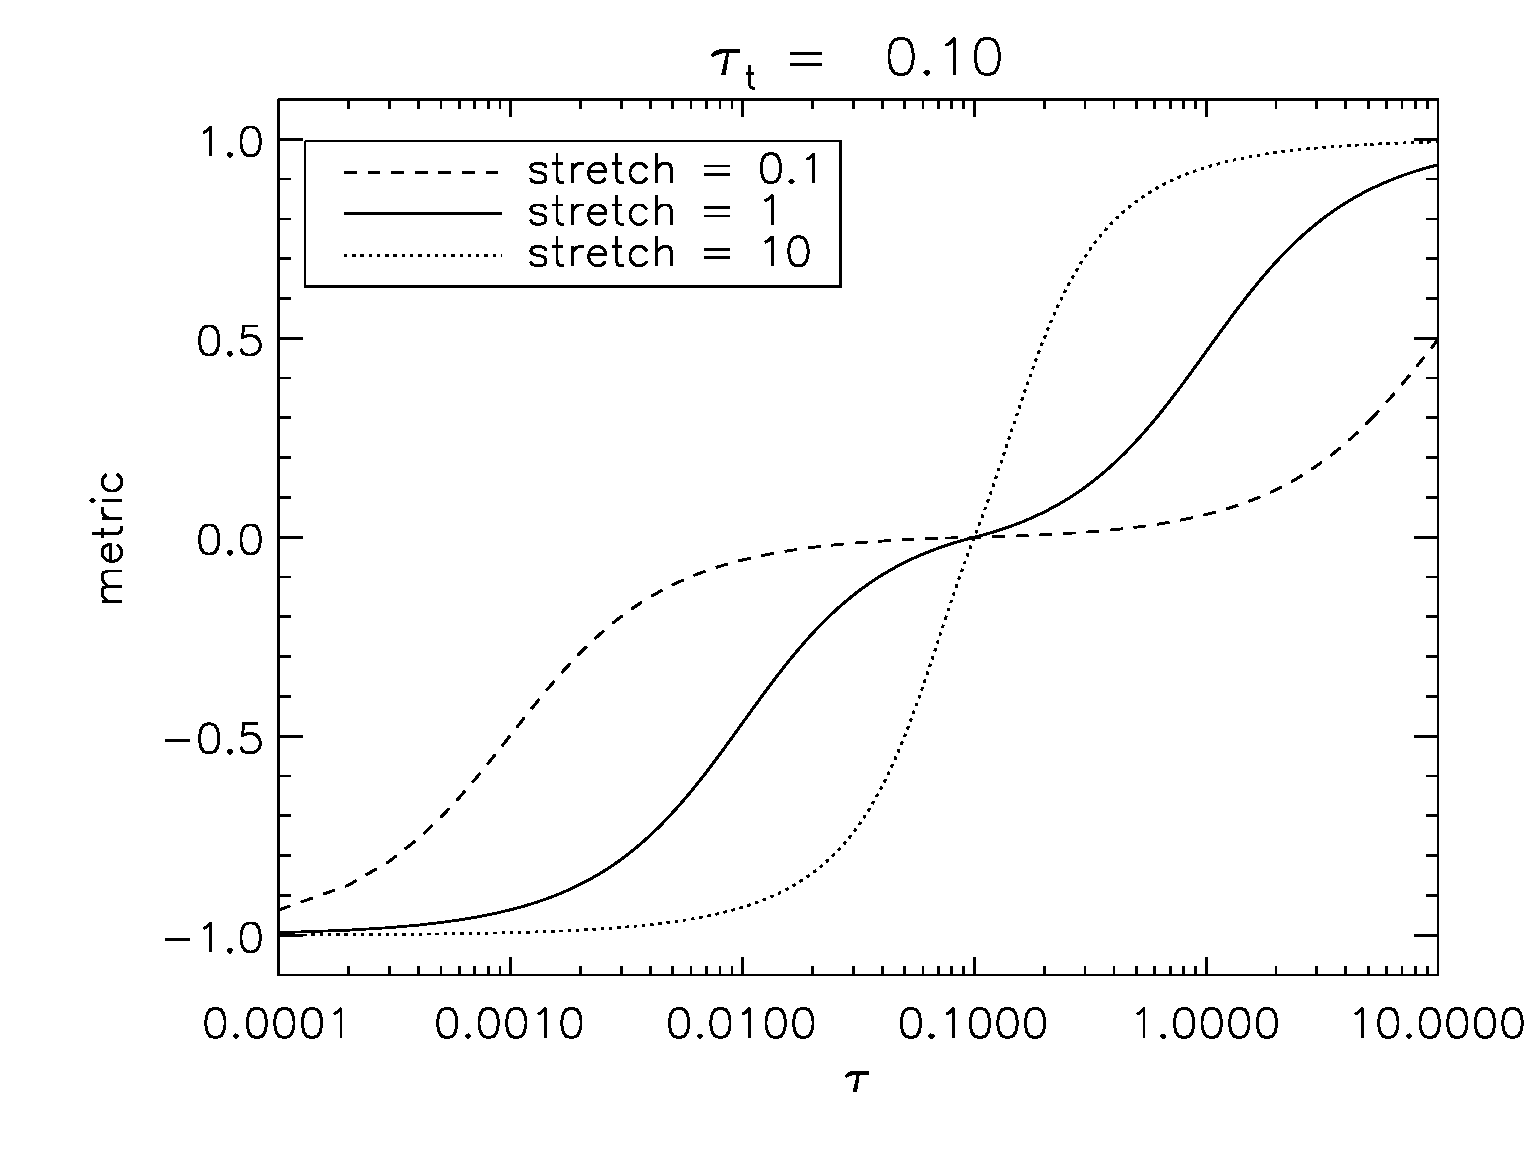
\includegraphics[width=\linewidth]{tau2metric_new.ps}
\end{center}

\paragraph{\texttt{tau\_thres}}

The usage of \texttt{tau\_thres} is described above.  It should divide
``high'' and ``low'' optical depths.  A typical value is 0.1.

\paragraph{\texttt{stretch}}

The \texttt{stretch} keyword assigns values for \texttt{stretch1} and
\texttt{stretch2}.  The usage is described above.

\paragraph{\texttt{npoint}}

The \texttt{npoint} keyword assigns values for \texttt{npoint1} and
\texttt{npoint2}.  There are \texttt{npoint1} optical depth bins for
$\texttt{x} < \texttt{tau\_thres}$ and \texttt{npoint2} optical depth
bins for $\texttt{x} > \texttt{tau\_thres}$

\paragraph{\texttt{nscatter}}

The \texttt{nscatter} keyword specifies the number of scattering bins
to use.

\subsection{The Sounding Input File}

This file is specified in the run file using the input\_file keyword.
It contains two blocks: the SOUNDING\_INFO block and the
PARAMETER\_DEFINITION block.

\subsubsection{The SOUNDING\_INFO block}

\paragraph{\texttt{spectrum\_file}}

The \texttt{spectrum\_file} specifies the spectrum data for the retrieval.
This can refer either the the output of the forward model or an L1B HDF file.

\paragraph{\texttt{range\_file}}

The \texttt{range\_file} specifies which l1b files should be read.

\paragraph{\texttt{soundinginfo\_file}}

The \texttt{soundinginfo\_file} specifies the scene date and location.

\paragraph{\texttt{sounding\_number}}

The \texttt{sounding\_number} specifies the sounding within L1B and ECMWF HDF
  files that should be used. The index is 1-based, so if you use \texttt{hdfview} to
	view HDF files, remember that \texttt{hdfview} uses 0-based indicies. This means that
	if you want the data shown at index 4 via \texttt{hdfview}, you'll need to specify 5
	here.

\paragraph{\texttt{frame\_number}}

The \texttt{frame\_number} specifies the frame within L1B and ECMWF HDF
  files that should be used. The index is 1-based, so if you use \texttt{hdfview} to
	view HDF files, remember that \texttt{hdfview} uses 0-based indicies. This means that
	if you want the data shown at index 4 via \texttt{hdfview}, you'll need to specify 5
	here.

\subsubsection{The PARAMETER\_DEFINITION block}

This block contains blocks for each element in the state vector.  The
\texttt{aerosol\_types}, \texttt{albedo\_types}, and
\texttt{retrieval\_vector} keywords should be defined outside of the
sub-blocks.

Each of the blocks contained here may use the following keywords:

\begin{tabular}{|l|p{3.75in}|}
\hline
\texttt{name}  &Name used for the column label in matrix files that are read in \\
\texttt{a\_priori} & Filename containing \textit{a priori\/} values.\\
\texttt{first\_guess}      & Filename containing first guess profiles.  If not present, \textit{a priori\/} values are used.\\
\texttt{covariance}      & Covariance matrix\\
\texttt{retrieval\_indices}      & list of retrieval indices, given as individual indices or a range.  1 2 3:11 12 is equivalent to 1:12, which means 1 through 12.\\
\texttt{perturb}      & Perturbations used for finite difference jacobians.\\
\hline
\end{tabular}


\paragraph{HDF Input Files}

\texttt{a\_priori} and \texttt{first\_guess} typically refert to matrix
	files.  However, they may refer to either an L1B or ECMWF HDF file for
	certain variables as described below:

\begin{tabular}{|l|l|l|}
\hline
Block &Variable &HDF File type \\
\hline
GAS &H20 &ECMWF \\
SURFACE\_PRESSURE &PSURF &ECMWF \\
TEMPERATURE &T &ECMWF \\
INSTURMENT &DISP &L1B \\
INSTURMENT &ILS &L1B* \\
\hline
\end{tabular}

* Note that for the ILS, you must always have an ASCII .dat file because
certain variables not available in L1B HDF files are are read from the 
headers of the ASCII file. To specify an L1B file for the ILS, add a
'hdf\_file' header to the ASCII file that contains the path on an L1B
HDF file.

\paragraph{\texttt{aerosol\_types}}

The \texttt{aerosol\_types} lists the aerosol types (can be more than
one) to be used in this run.  Each name here must have a matching name
in an AEROSOL block later in the file.

\paragraph{\texttt{ground\_type}}

The \texttt{ground\_type} lists the ground type (only specify one) to
be used in this run.  Each name here must have a matching name in a
BRDF block later in the file.

\paragraph{\texttt{retrieval\_vector}}

The \texttt{retrieval\_vector} keyword lists the elements of the state
vector that are to be retrieved.  The \texttt{name} field of each
state vector element to be retrieved should be placed here.  For the
BRDF block, use the name for the whole BRDF block, and not the names
for the individual sub-blocks.

\paragraph{AEROSOL block}

The AEROSOL block contains the following keywords in addition to the
general ones specified above:

\begin{tabular}{|l|p{3.75in}|}
\hline
\texttt{mie\_file}  & Mie scattering parameters \\
\texttt{moment\_file}  & Aerosol phase function moments\\
\texttt{retrieval\_mode}  & can be LINEAR or LOGARITHMIC\\
\hline
\end{tabular}

\paragraph{BRDF block}

A BRDF type can have spectrally dependent and independent parameters.
Each type is contained in either the SPECTRALLY\_DEPENDENT or
SPECTRALLY\_INDEPENDENT sub-blocks.  

\begin{tabular}{|l|p{3.75in}|}
\hline
\texttt{type} & BRDF type - currently either lambert or coxmunk.
Specify this outside of the sub-blocks.\\
\texttt{num\_parameters}   & number of parameters used to fit the function\\
\texttt{num\_coefficients} & number of polynomial coefficients for
each parameter.  Only used in the spectrally dependent sub-block.\\
\hline
\end{tabular}


\paragraph{GAS block}
The GAS block contains the following keywords in addition to the general ones specified above:

\begin{tabular}{|l|p{3.75in}|}
\hline
\texttt{hitran\_index} & HITRAN index of the gas - not used\\
\texttt{isotope}       & isotope label (e.g. 626 for O$^{16}$C$^{12}$O$^{16}$) - not used\\
\texttt{absco\_file}   & absorption coefficient file name\\
\texttt{scale\_parameters} & Four values: \textit{a priori}, initial guess, perturbation, covariance\\
\hline
\end{tabular}

The \texttt{scale\_parameters} keyword is optional.  If present, a single scaling factor will be retrieved.  This scaling factor is multiplied by the profile to give the best fit.

\paragraph{INSTRUMENT block}

A separate INSTRUMENT block needs to be specified for each instrument parameter with the \texttt{type} keyword.

\begin{tabular}{|l|p{3.75in}|}
\hline
\texttt{type} & CHANNELING, CONTINUUM, DISPERSION, GHOST, ILS, STRAY\_LIGHT, or ZERO\_LEVEL\\
\hline
\end{tabular}

\paragraph{SOLAR block}

\begin{tabular}{|l|p{3.75in}|}
\hline
\texttt{solar\_linelist} & list of solar lines, output from GFIT\\
\hline
\end{tabular}

\paragraph{SURFACE\_PRESSURE block}

The SURFACE\_PRESSURE block has no keywords specific to it.

\paragraph{TEMPERATURE block}

\begin{tabular}{|l|p{3.75in}|}
\hline
\texttt{scale\_parameters} & Four values: \textit{a priori}, initial guess, perturbation, covariance\\
\hline
\end{tabular}

As in the GAS block, the \texttt{scale\_parameters} keyword is optional.

\appendix

\section{SSH Tunneling}

The JPL firewall restricts access to most of the services on
nephthys.  External users can use SSH to connect, but the web and
subversion servers are not accessible.  SSH tunneling can be used to
``tunnel'' the web and subversion connections through SSH.

On the Colorado State system, I have created a file called
\texttt{config} in \texttt{/home/nair/.ssh} containing:

\begin{verbatim}
  Host nephthys
     ForwardX11   yes
     HostName     nephthys.jpl.nasa.gov
     LocalForward 20000 137.78.162.28:80
     LocalForward 20443 137.78.162.28:443
     ServerAliveInterval 600
     User         hnair
\end{verbatim}

This sets up ports on your local machine
(e.g. coral.atmos.colostate.edu) that are redirected to ports on
nephthys.  For example, the web server on nephthys is active on port
80.  The line

\begin{verbatim}
  LocalForward 20000 137.78.162.28:80
\end{verbatim}

redirects port 80 on IP address 137.78.162.28 (you can also use
127.0.0.1, since this is how a unix machine refers to itself) to port
20000 on coral.  The subversion server is active on port 443 on
nephthys.  This gets mapped to port 20443 on coral.

So to access the OCO Wiki, create an \texttt{\${HOME}/.ssh/config}
file like the one above (using your username, of course), and then
\texttt{ssh nephthys}.

Now if you open up a browser and point it to
\texttt{http://localhost:20000/$\sim$hnair/OCOWiki/}, you should see the
wiki page.

If you close the ssh connection to nephthys and try to reload the wiki
page, you will get an error.

To list the contents of the subversion repository:

\begin{verbatim}
  svn ls https://localhost:20443/oco/alg
\end{verbatim}

You should see:

\begin{verbatim}
  L2_Contrib/
  L2_EXE/
  L2_Support/
  L2_Tests/
\end{verbatim}

\section{Using \texttt{subversion}}

All of the OCO code, including that developed by the GDS, is managed
using \texttt{subversion}.  There are only a few commands you really
need to know:

\begin{tabular}{|l|l|l|}
\hline
Command & Short form & Description \\
\hline
\texttt{svn checkout} & \texttt{svn co} & Checkout a working copy\\
\texttt{svn update} & \texttt{svn up} & Update working copy\\
\hline
\texttt{svn diff} & \texttt{svn di} & Show differences between two versions\\
\texttt{svn list} & \texttt{svn ls} & List directory contents\\
\texttt{svn log} & \texttt{svn log} & Print commit log messages\\
\texttt{svn revert} & \texttt{svn revert} & Revert working copy to
original version\\
\texttt{svn status} & \texttt{svn st} & Print status of working copy\\
\hline
\end{tabular}

\section{Using \texttt{screen}}

\texttt{screen} is an enormously useful program that is included on
most modern Unix systems (including OS~X).  It creates a terminal
session that can be detached and reattached at any time.  What this
means is that you can set a job running inside of a screen session,
detach it and go home, and then reattach it from home to check on its
progress.

It is also very useful for setting up ssh tunnels.  On the Colorado
State computers, I ssh to nephthys using a screen session, and then
detach.  When I don't need the tunnel anymore, I reattach the screen
and log out.

\texttt{screen} creates a new screen. \texttt{screen -r} reattaches a
detached screen.  Basic commands within screen are:

\begin{tabular}{|l|l|l|}
\hline
Key sequence & Name & Description\\
\hline
\texttt{ctrl-a ''} & windowlist & Show the list of windows\\
\texttt{ctrl-a A} & title & Name this window\\
\texttt{ctrl-a c} & create & Create a new window\\
\texttt{ctrl-a d} & detach & Detach the session\\
\texttt{ctrl-a n} & next & Go to the next window \\
\texttt{ctrl-a p} & previous & Go to the previous window\\
\hline
\end{tabular}

\section{Sample Files}

\subsection{Matrix File}

This is a file that can specified as an a\_priori or first\_guess file in a GAS parameter block, and/or as the pressure\_file in the oco\_l2.run file.

\begin{verbatim}
begin HEADER
  File_ID = "Atmospheric State - Lauder, July"
  File_Creation = "Tue Oct 10 15:35:10 2006"
  File_Type = "Matrix"
  Num_Rows =      12
  Num_Columns =       5
  Labels = "Pressure" "T" "H2O" "CO2" "O2"
  Units  = "Pa" "K" "VMR" "VMR" "VMR"
end HEADER

# Pressure T H2O CO2 O2
# (Pa)             (K)     (VMR)           (VMR)   (VMR)
      100.000      245.360  5.11594e-06  0.000368931 0.2095
      7000.00      221.815  3.23449e-06  0.000374329 0.2095
      10000.0      221.558  2.92339e-06  0.000375367 0.2095
      20000.0      219.754  5.56769e-06  0.000375895 0.2095
      35000.0      228.431  0.000170962  0.000376235 0.2095
      45000.0      240.849  0.000621730  0.000376108 0.2095
      55000.0      252.295   0.00155334  0.000375761 0.2095
      65000.0      261.206   0.00281429  0.000375366 0.2095
      75000.0      266.232   0.00401206  0.000375146 0.2095
      85000.0      270.859   0.00556349  0.000375098 0.2095
      95000.0      277.408   0.00669547  0.000374922 0.2095
      105000.      283.154   0.00687684  0.000374915 0.2095
\end{verbatim}


\subsection{Run File}
\begin{verbatim}
# These are useful to keep at the top, as you probably want to catch
# error messages as this file is being parsed.  Choices for verbosity
# are are DEBUG, INFO, WARNING, ERROR, FATAL.
verbosity           = DEBUG
log_file            = oco_l2.log


### Input file for this run
input_file     = oco_l2.inp

### Run flags
append = True
control_flag = TRUE
zero_azimuth = TRUE

### Instrument parameters
noise_file                = in/instrument/noise.dat
num_spectrometers         = 3
num_channeling_parameters = 0
num_continuum_parameters  = 0
num_dispersion_parameters = 3
num_ghost_parameters      = 0

num_ils_parameters        = 1

# describe each ils parameter by a polynomial with this many
# coefficients (1 means each parameter is constant, 2 linear, etc.)
num_ils_wndepend          = 1  

num_stray_parameters      = 0
num_zero_level_parameters = 1

### Define Spectral Windows
spectral_window_file = oco_l2.win
spectral_windows = 1 # Spectrometer 1
spectral_windows = 2 # Spectrometer 2
spectral_windows = 3 # Spectrometer 3
#bin_windows = 1 2 3

### Run parameters
num_levels                = 12
num_solar_parameters      = 4

target_species            = CO2
pressure_file = in/scene/atmosphere/pressure.dat # Reads the column labeled PRESSURE

jacobian_mode  = ANALYTIC
#jacobian_mode  = FINITE_DIFFERENCE

#run_mode       = FORWARD_MODEL # Run a single iteration of the forward model 
run_mode       = JACOBIAN_ONLY # Calculate jacobians, don't do a retrieval
#run_mode      = RETRIEVAL     # Run a full retrieval
#run_mode      = SOLAR         # Retrieve Solar model parameters

# Forward model parameters
absco_path    = /state/partition1/ABSCO/v2.0.1/
polarization  = false             # Turn on polarization
spec_path     = in/l1b/spec/OCO/  # Path of l1b spectrum file
streams       = 8                 # Number of streams that RADIANT will use

single_scatter_correction = false
delta_m_scaling = true

interpolation = 100 100 100       # resolution of fine grid/calculated grid
ils_cycle = 6 6 6
apo_m = 1
nlines = 20585
reclen = 101
points_sun = 10000

# retrieval parameters
max_divergence    = 30   # stop after this number of diverging steps
max_iterations    = 30   # stop after this many iterations
max_chi2          = 1.0  # fail convergence if chi2 > max_chi2
lm_gamma          = 0.0  # Levenberg-Marquardt gamma 
scale_convergence = 1.0  # converged if d_sigma_sq < scale_convergence * len_sv
final_rad = t t t f f f
do_error = True tRue f false F

num_diodes = 1024 1024 1024

# output files

# all output files will go here, except log file
output_path   = out/
result_file   = results.dat     # state vector output file name
out_info_file = out_info.dat    # additional output file
output_each_iteration = FALSE   # save radiances & jacobians at each iteration

# Save jacobians and covariances in this dir for offline error
# analysis.  If not present, no files will be saved.
control_path      = control1/         # underneath output_path
controlsub_path   = o_l/              # underneath control_path
control_file      = control_file.dat  # in control_path

# Atmosphere file
atmos_file = atmosphere.dat

### Anything below this is not implemented yet

# All diagnostic files go here.  If not present, no files will be created.
diagnostic_path     = diagnostics/  # underneath output_path
high_res_spectra    = TRUE          # create high-resolution spectra files
save_jacobians      = TRUE          # save jacobian files
solar_transmittance = TRUE
\end{verbatim}

\subsection{Input File}

\begin{verbatim}
# Lauder, July
# soundinginfo_file = in/l1b/soundinginfo_la_Jul1.dat

# A priori for gas/temperature, psurf, brdf, and aerosol type:
# a_priori          = in/scene/atmosphere/atmosphere_la_Jul1.dat
# a_priori          = in/scene/psurf/psurf_la_Jul1.dat
# a_priori          = in/scene/frost.dat
# mie_file          = ./in/scene/aerosol/vij_2.mie
# moment_file       = ./in/scene/aerosol/vij_2.mom

begin SOUNDING_INFO

  range_file   = in/l1b/range.dat
  soundinginfo_file = in/l1b/soundinginfo_la_Jul1.dat

end SOUNDING_INFO

### Define Initial State and Retrieval Parameters
begin PARAMETER_DEFINITION

  aerosol_types = TROP_01 STRAT 
  ground_type  = frost

  retrieval_vector = ALBEDO CO2

# The following blocks define the retrieval vector.
  begin GAS
    name              = CO2
    hitran_index      = 2
    isotope           = 626
    a_priori          = in/scene/atmosphere/atmosphere_la_Jul1.dat
    absco_file        = co2_4700_6500_v21.abs
# If first guess is not specified, a priori will be used
#   first_guess       = ./in/scene/atmosphere/atmosphere_fg.dat
    perturb           = ./in/scene/atmosphere/atmosphere_perturb.dat
    covariance        = ./in/covariance/co2_cov.dat
    retrieval_indices = 1:12       # retrieve levels 1 through 12
# retrieve single scaling factor instead of a profile
# A priori, initial guess, perturbation, covariance
#    scale_parameters = 1.0 1.0 0.01 0.1   
  end GAS

  begin GAS
    name              = H2O
    hitran_index      = 1
    isotope           = 161
    a_priori          = in/scene/atmosphere/atmosphere_la_Jul1.dat
    perturb           = ./in/scene/atmosphere/atmosphere_perturb.dat
    absco_file        = h2o_4700_6500_v21.abs
    covariance        = ./in/covariance/h2o_cov.dat
    retrieval_indices = 1:12       # retrieve levels 1 through 12
  end GAS

  begin GAS
    name              = O2
    hitran_index      = 7
    isotope           = 66
    a_priori          = in/scene/atmosphere/atmosphere_la_Jul1.dat
    absco_file        = o2_12745_13245_v21.abs
  end GAS

# Surface pressure is not being retrieved but there's no harm in
# putting covariance and pertubation files here
  begin SURFACE_PRESSURE
    name              = PSURF
    a_priori          = in/scene/psurf/psurf_la_Jul1.dat
    covariance        = ./in/covariance/psurf_cov.dat
    perturb           = ./in/scene/psurf/psurf_perturb.dat
    retrieval_indices = 1
  end SURFACE_PRESSURE

  begin TEMPERATURE
    name              = T
    a_priori          = in/scene/atmosphere/atmosphere_la_Jul1.dat
    covariance        = ./in/covariance/t_cov.dat
    perturb           = ./in/scene/atmosphere/atmosphere_perturb.dat
    retrieval_indices = 1:12 
# retrieve single additive factor instead of a profile
# A priori, initial guess, perturbation, covariance
#    scale             = 0 0 2 10
  end TEMPERATURE

  begin AEROSOL
    name              = TROP_01
    a_priori          = ./in/scene/aerosol/aerosol.dat
    covariance        = ./in/covariance/aero_od_01_cov.dat
    mie_file          = ./in/scene/aerosol/vij_2.mie
    moment_file       = ./in/scene/aerosol/vij_2.mom
    perturb           = ./in/scene/aerosol/aerosol_perturb.dat
    retrieval_indices = 1:12 
  end AEROSOL

  begin AEROSOL
    name              = STRAT
    a_priori          = ./in/scene/aerosol/aerosol.dat
    mie_file          = ./in/scene/aerosol/strat.mie
    moment_file       = ./in/scene/aerosol/strat.mom
  end AEROSOL

 begin BRDF
    name        = frost
    type        = lambert
    begin SPECTRALLY_DEPENDENT
      num_parameters    = 1 
      num_coefficients  = 2
      name              = albedo
      a_priori          = ./in/scene/ground/frost.dat
      covariance        = ./in/covariance/lambert_cov.dat
      perturb           = ./in/scene/ground/lambert_perturb.dat

# Don't comment these out; just remove the indices if you don't want
# to retrieve them.  
      retrieval_indices = 1 2   # spectrometer 1, parameter 1 coefficients
      retrieval_indices = 1 2   # spectrometer 2, parameter 1 coefficients
      retrieval_indices = 1 2   # spectrometer 3, parameter 1 coefficients
    end SPECTRALLY_DEPENDENT
  end BRDF

  begin INSTRUMENT
    type              = DISPERSION
    name              = DISP
    a_priori          = ./in/instrument/dispersion.dat
    covariance        = ./in/instrument/dispersion_cov.dat
    perturb           = ./in/instrument/dispersion_perturb.dat

# Don't comment these out; just remove the indices if you don't want
# to retrieve them.  
    retrieval_indices = 1 2 3       # spectrometer 1
    retrieval_indices = 1 2 3       # spectrometer 2
    retrieval_indices = 1 2 3       # spectrometer 3
  end INSTRUMENT

  begin INSTRUMENT
    type              = ZERO_LEVEL
    name              = ZERO
    a_priori          = ./in/instrument/zero_level.dat
    covariance        = ./in/instrument/zero_level_cov.dat
    perturb           = ./in/instrument/zero_level_perturb.dat

# Don't comment these out; just remove the indices if you don't want
# to retrieve them.  
    retrieval_indices =       # spectrometer 1
    retrieval_indices =       # spectrometer 2
    retrieval_indices =       # spectrometer 3
  end INSTRUMENT

  begin INSTRUMENT
    type              = ILS
    name              = ILS
    a_priori          = ./in/instrument/ils.dat
    covariance        = ./in/instrument/ils_cov.dat
    perturb           = ./in/instrument/ils_perturb.dat

# Don't comment these out; just remove the indices if you don't want
# to retrieve them.  These lines are read in a loop like this:
# do i = 1, n_spec
#   do j = 1, num_ils_parameters 
#     read num_ils_wndepend polynomial coefficients for each ils parameter
#   end do
# end do
    retrieval_indices =       # spectrometer 1, parameter 1 coefficients
    retrieval_indices =       # spectrometer 2, parameter 1 coefficients
    retrieval_indices =       # spectrometer 3, parameter 1 coefficients
  end INSTRUMENT

  begin SOLAR
    a_priori       = ./in/solar/solar.dat
    covariance     = ./in/solar/solar_cov.dat
    perturb        = ./in/solar/solar_perturb.dat
    solar_linelist = ./in/solar/solar_di.h92
#    retrieval_indices = 1:4
  end SOLAR

end PARAMETER_DEFINITION
\end{verbatim}

\subsection{Spectral Windows File}

\begin{verbatim}

begin WINDOW
      id = 1
      name = O2 A Band
      units = wavelength
      range = 0.755 0.785
      species = O2

      # Binning parameters
      tau_thres = 0.2
      stretch   = 12 1
      npoint    = 20 7
      nscatter  = 3

end WINDOW

begin WINDOW
      id = 2
      name = Weak CO2
      units = wavelength
      range = 1.58 1.65
      species = CO2 H2O

      tau_thres = 0.1
      stretch   = 20 6
      npoint    = 20 5
      nscatter  = 3
end WINDOW

begin WINDOW
      id = 3
      name = Strong CO2
      units = wavelength
      range = 2.03 2.09
      species = CO2

      tau_thres = 0.2
      stretch   = 12 4
      npoint    = 20 5
      nscatter  = 3
end WINDOW

\end{verbatim}

\end{document}
